\section{Programmierumgebung finden}
\setauthor{Elisa Kaltenberger}

Für die vorliegende Diplomarbeit wurde die Unity Engine gegenüber der Unreal Engine aus mehreren, 
auf das Projekt zugeschnittenen Gründen ausgewählt. Die Entwicklung einer 3D-VR-Simulation erforderte 
eine sorgfältige Abwägung, wobei Unity insgesamt die bessere Eignung aufwies.
(Quelle1, Quelle2)

Der entscheidende Faktor war die gewohnte Programmierbasis. Da die schulische Ausbildung ausschließlich 
auf Java ausgerichtet war, bot Unity mit der Programmiersprache C-Sharp einen idealen und höchst effizienten 
Übergang. Die Ähnlichkeit der Sprachen in Syntax und objektorientierten Konzepten ermöglichte eine 
unmittelbare Übertragung des bestehenden Wissens auf die Engine-Programmierung. Dadurch war es möglich, 
den Fokus von Beginn an auf die spezifischen Herausforderungen der VR-Programmierung zu legen. Zu diesen 
Herausforderungen zählen beispielsweise Interaktion, Bewegung und die Optimierung der Performance für VR. 
Die Verwendung der Unreal Engine, die eine komplexere C++-Sprache sowie ein völlig anderes Blueprint-System 
erfordert hätte, hätte zu einem erheblichen Mehraufwand an Lernzeit geführt und somit wertvolle Zeit für die 
inhaltliche Entwicklung der Simulation in Anspruch genommen.
(Quelle1, Quelle3)

Zweitens ist Unity im Bereich VR/XR besonders gut aufgestellt und zugänglich. Über das XR Interaction Toolkit 
und die OpenXR-Unterstützung werden von Unity standardisierte und gut dokumentierte Frameworks speziell für die 
VR-Entwicklung angeboten. Diese Tools abstrahieren plattformspezifische Schwierigkeiten und ermöglichen einen 
effizienten Einstieg in die Entwicklung von Interaktionen für VR-Controller. Obwohl Unreal Engine ebenfalls 
über ausgeprägte VR-Fähigkeiten verfügt, wird der Einstieg in die VR-Interaktionsprogrammierung mit Unity 
aufgrund der hochwertigen, offiziellen Plugins oft als direkter und schulprojektfreundlicher empfunden.
(Quelle1, Quelle2, Quelle3)

Die Performance-Charakteristik wurde dahingehend modifiziert, dass eine bessere Passung zum Projekt erzielt 
wurde. Für eine stabile VR-Simulation ist eine hohe und konstante Framerate (FPS) von entscheidender Bedeutung, 
um das Auftreten von Motion Sickness zu vermeiden. Unity-Projekte werden als vergleichsweise ressourcenschonend 
und gut optimier- sowie kontrollierbar angesehen, was für den überschaubaren Umfang einer schulischen Simulation 
vorteilhaft war. Obwohl die Unreal Engine häufig eine beeindruckendere Grafik erzeugt, weist sie in zahlreichen 
Szenarien einen höheren "Basis-Overhead" auf und erfordert eine leistungsstärkere Hardware. Im Rahmen eines 
exemplarischen Simulationsprojekts, das sich durch eine starke Fokussierung auf die inhaltliche Interaktion 
auszeichnete, wurde Unity als die Lösung identifiziert, die ein optimales Verhältnis zwischen visueller Qualität 
und garantierter Leistung der verfügbaren Hardware aufwies. Dies steht im Gegensatz zu fotorealistischen 
Visualisierungen, die bei diesem Projekt nicht im Vordergrund standen.
(Quell1, Quelle2)

\section{Welt einrichten}
\subsection{Überlegung der Hindernisse}
Zunächst wurden die signifikanten Hindernisse für Rollstuhlfahrende identifiziert und einer Analyse unterzogen. 
Auf dieser Grundlage wurde anschließend die VR-Welt gestaltet, um ein möglichst realistisches und zugleich 
bestmögliches Ergebnis zu erzielen.

Für Menschen mit Mobilitätseinschränkungen kann die Nutzung eines Bankautomaten eine Herausforderung darstellen. 
In einer signifikanten Anzahl von Fällen sind die Automaten zu hoch angebracht, was dazu führt, dass sowohl der 
Bildschirm als auch das Tastenfeld nur mit einem hohen Aufwand erreicht werden können. In vielen Fällen ist die 
zur Verfügung stehende Bewegungsfläche vor dem Automaten unzureichend. Ein zusätzliches Problem stellt der 
Sichtschutz dar, da die seitlichen Schutzblenden oder Abdeckungen in der Regel für stehende Personen konzipiert sind.

Eine Bordsteinkante stellt für Rollstuhlfahrer*innen im Alltag eine signifikante Barriere dar. Die Höhe der 
Bordsteine hat einen signifikanten Einfluss auf die Fähigkeit der Verkehrsteilnehmer, die Straße selbstständig zu 
überqueren. Selbst geringfügige Höhenunterschiede können eine Gefahr darstellen, da die Räder im Rollstuhl hängen 
bleiben oder das Gefährt umkippen kann. Abgesenkte Bordsteine werden häufig als unzureichend gestaltet wahrgenommen 
oder deren Nutzung wird durch parkende Autos, Fahrräder oder Baustellen erschwert. Bei Niederschlag kommt es zu 
einer Wasseransammlung, was das Überfahren zusätzlich erschwert.

Des Weiteren ist festzustellen, dass Pflastersteine problematisch sind. Die unebene Oberfläche des Produkts 
führt zu einer signifikanten Erschütterung, die sich negativ auf die körperliche Verfassung auswirken kann. 
Es wurde beobachtet, dass insbesondere die kleinen Vorderräder des untersuchten Objekts in Fugen oder abgesackten 
Steinen hängen bleiben können. Bei Nässe oder Glätte können Pflastersteine eine erhöhte Rutschgefahr aufweisen, 
was das Unfallrisiko signifikant erhöhen kann. Zudem ist ein deutlich höherer Kraftaufwand erforderlich, um auf 
diesen Wegen zu reisen, was die Autonomie der Fortbewegung erheblich einschränkt.

\subsection{Erster Prototyp}
Der erste Prototyp der VR-Welt wurde in Unity erstellt, um die zuvor identifizierten Hindernisse für 
Rollstuhlfahrende zu simulieren. Dabei wurden verschiedene Umgebungen modelliert, die typische Herausforderungen 
im Alltag darstellen, wie z.B. Bankautomaten, Bordsteinkanten und Pflastersteine.

In der ersten konkreten Umsetzungsphase des Projekts wurde ein strategischer Fokus auf Funktionalität und 
Nutzerperspektive gelegt. Hierzu wurde bewusst auf den Import komplexer, fertiger 3D-Assets verzichtet. 
Unter „Assets“ versteht man in diesem Kontext vollständig texturierte Modelle wie Gebäude, Autos oder 
detaillierte Oberflächenmaterialien, die üblicherweise für die visuelle Vollendung einer virtuellen 
Umgebung genutzt werden.

Stattdessen wurde eine minimalistische, abstrakte Testumgebung erstellt, die auch als Whitebox- oder 
Greybox-Prototyp bezeichnet wird. Die vorliegende Struktur besteht ausschließlich aus einfachen 
geometrischen Grundkörpern, die direkt innerhalb der Unity Engine erzeugt und arrangiert wurden. 
Die gesamte Szene wurde folglich in einer reduzierten, häufig einfarbigen oder grob gerasterten 
Darstellung präsentiert.
(Quelle ITP Buch)

Das primäre und ausschließliche Ziel dieser Phase war die funktionale Validierung der zentralen Hindernisse 
ausschließlich aus der spezifischen Perspektive eines Rollstuhlfahrers. Es ging nicht um realistische 
Darstellung, sondern um die Beantwortung essenzieller technischer und konzeptioneller Fragen: Werden die 
Hindernisse aus der festgelegten Sitzhöhe korrekt und eindeutig wahrgenommen? Funktioniert die physikalische 
Kollisionserkennung an Bordsteinen und Kanten wie intendiert? Löst die Platzierung eines simulierten 
Bankautomaten das gewünschte Interaktionsproblem (Unerreichbarkeit, eingeschränkte Sicht) aus? Wie fühlt 
sich die Bewegung über ein Feld unebener Pflastersteine in der reinen Gameplay-Logik an? 

\begin{figure}
    \centering
    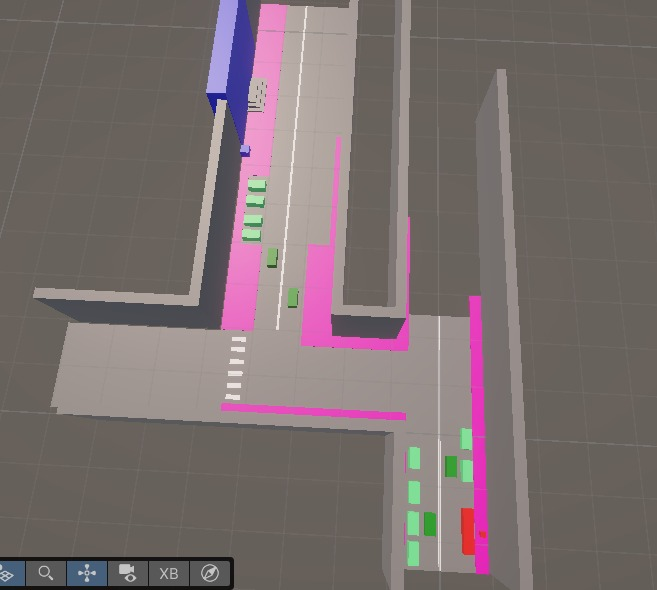
\includegraphics[scale=0.5]{pics/prototyp-welt.jpg}
    \caption{Prototyp der VR-Welt mit Hindernissen für Rollstuhlfahrende}
    \label{fig:vr-world:prototyp}
\end{figure}

\subsection{Welt gestalten}
Nach erfolgreicher Einrichtung der Testumgebung wurde ein umfangreiches Asset-Paket einer realen Stadt 
ausgewählt und heruntergeladen. Im Anschluss daran wurden die einzelnen Gebäude manuell aus dem Paket 
extrahiert, separat aufbereitet und in die virtuelle Realität integriert. Um die Szenerie lebendiger 
und authentischer wirken zu lassen, wurden zusätzliche Elemente wie detailreiche Gehsteige, verschiedene 
Fahrzeugmodelle sowie ein vollständiges Straßennetz systematisch hinzugefügt.

Die Modellierung, Texturierung und Integration der weiteren ästhetischen Komponenten, welche nicht durch 
das Asset-Paket abgedeckt waren, erfolgte individuell. Im Anschluss wurden diese in die virtuelle 
Umgebung implementiert. Der kreative und technische Prozess, der zur Schaffung einer immersiven, 
kohärenten und visuell ansprechenden VR-Landschaft führte, ist als erfolgreich zu betrachten.

\begin{figure}
    \centering
    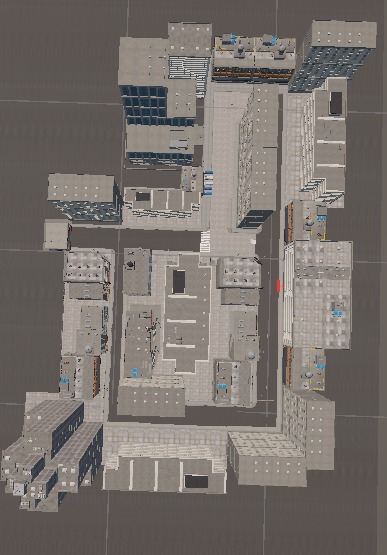
\includegraphics[scale=0.7]{pics/umgesetzte-welt.jpg}
    \caption{Umgesetzte VR-Welt mit Hindernissen für Rollstuhlfahrende}
    \label{fig:vr-world:umgesetzte-welt}
\end{figure}


